\documentclass{standalone}
\usepackage{tikz}
\usepackage{pgfplots}
\pgfplotsset{compat=1.16}

\begin{document}
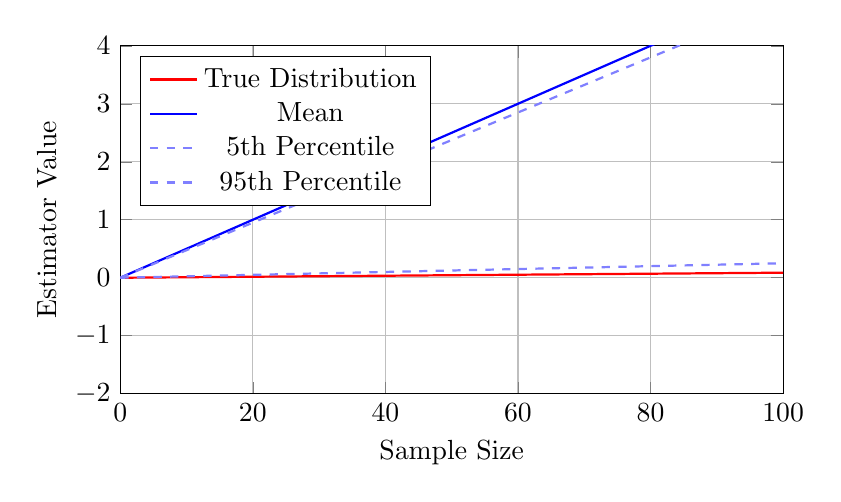
\begin{tikzpicture}
    \begin{axis}[
        xlabel={Sample Size},
        ylabel={Estimator Value},
        legend pos=north west,
        ymin=-2,
        ymax=4,
        xmin=0,
        xmax=100,
        ytick={-2,-1,0,1,2,3,4},
        xtick={0,20,40,60,80,100},
        grid=major,
        width=10cm,
        height=6cm
    ]
        % True distribution (red line)
        \addplot[domain=0:100, samples=100, thick, red] {sin(x/20)};
        \addlegendentry{True Distribution}

        % Mean (blue line)
        \addplot[domain=0:100, samples=100, thick, blue] {x/20};
        \addlegendentry{Mean}

        % 5th Percentile (blue dashed line)
        \addplot[domain=0:100, samples=100, thick, blue!50!white, dashed] {0.05*x/20};
        \addlegendentry{5th Percentile}

        % 95th Percentile (blue dashed line)
        \addplot[domain=0:100, samples=100, thick, blue!50!white, dashed] {0.95*x/20};
        \addlegendentry{95th Percentile}
    \end{axis}
\end{tikzpicture}
\end{document}